\subsubsection{XGBoost Results}

Following the methodology described earlier—specifically, performing grid search with cross-validation to tune hyperparameters—we found that the best values were: 500 trees, a maximum depth of 20, and a minimum child weight of 2. With these settings, an accuracy of 0.852 was achieved using only 50\% of the dataset for training. When the model was later trained using the entire training set, the accuracy increased to 0.86.

Table~\ref{tab:xgboost_classification_report} shows the classification report. It is worth highlighting that the model tends to predict the “Non-toxicity” class more frequently, as it has a higher recall compared to the positive (toxic) class, although its precision is lower. This indicates the presence of more false negatives, which also affects the recall of the positive class: more false negatives mean fewer true positives. To address this issue, a larger number of toxic examples could be included in the training data. Although this would create an imbalance, it would allow the model to better understand the class it is intended to detect and potentially improve its performance.

\begin{table}[htbp]
\centering
\caption{Classification report for XGBoost model on the test set.}
\label{tab:xgboost_classification_report}
\begin{tabular}{lcccc}
\toprule
\textbf{Class} & \textbf{Precision} & \textbf{Recall} & \textbf{F1-score} & \textbf{Support} \\
\midrule
0 (Non-toxic)   & 0.83 & 0.89 & 0.86 & 4626 \\
1 (Toxic)       & 0.89 & 0.83 & 0.86 & 4912 \\
\midrule
\textbf{Accuracy}       &      &      & 0.86 & 9538 \\
\textbf{Macro avg}      & 0.86 & 0.86 & 0.86 & 9538 \\
\textbf{Weighted avg}   & 0.86 & 0.86 & 0.86 & 9538 \\
\bottomrule
\end{tabular}
\end{table}

In Figure~\ref{fig:confusion_matrix_xgboost}, the model's confusion matrix can be observed. It reflects the quality of the model, showing a high concentration of true positives and true negatives. However, the accuracy is 86\%, and more than 1300 misclassified examples are observed in the test set. This implies that, in a production environment, there could be cases of toxicity that persist or non-toxicity cases that are unjustly censored.

\begin{figure}[H]
    \centering
    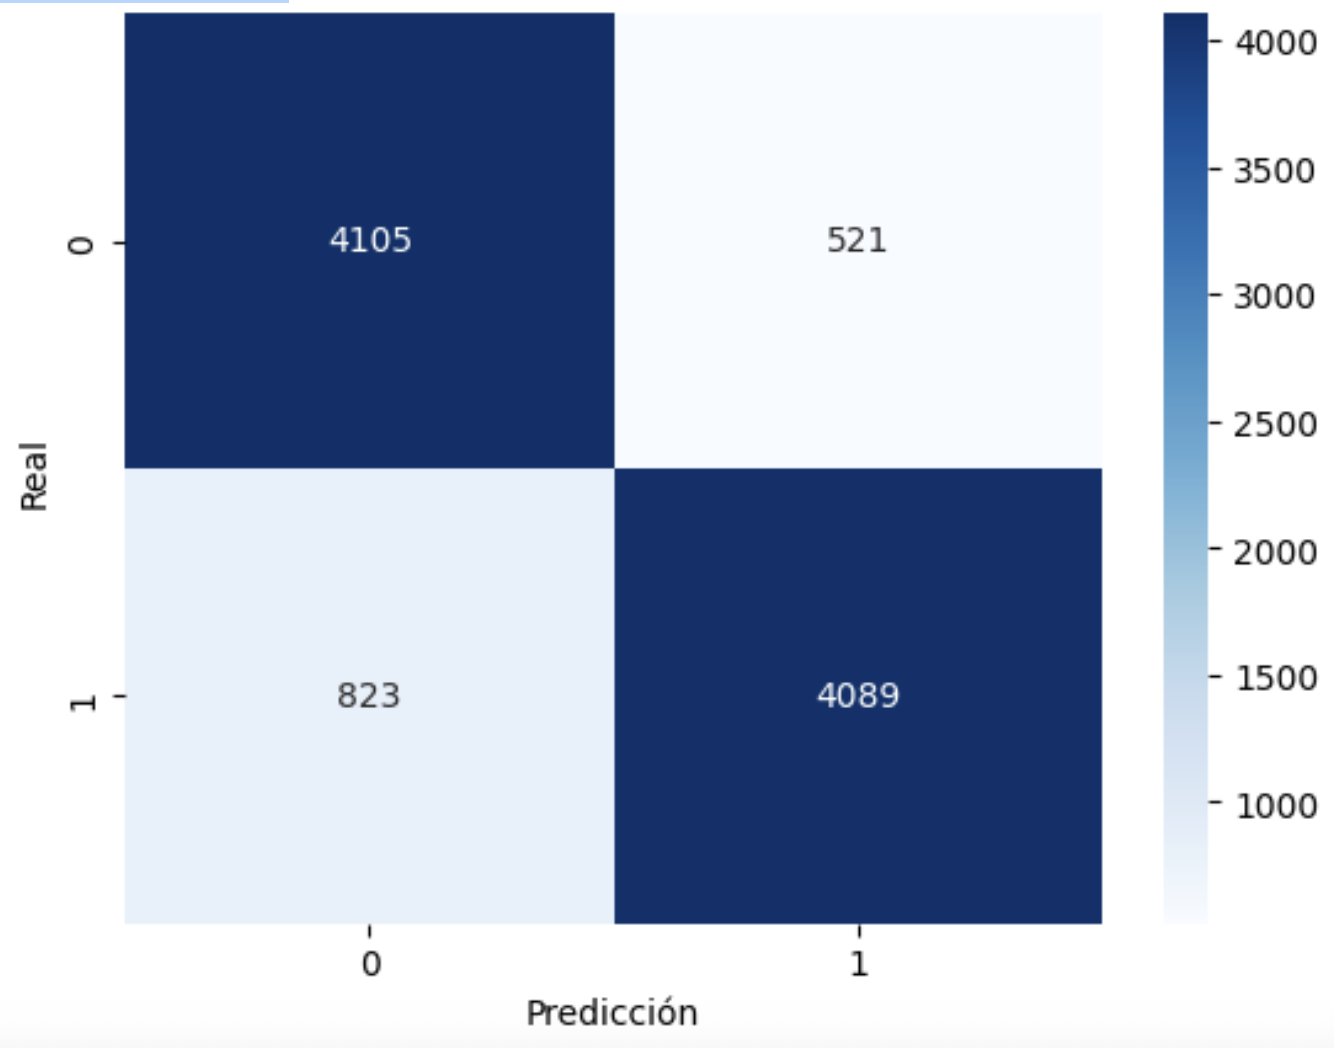
\includegraphics[width=0.45\textwidth]{images/confusion_matrix_xgboots.png} 
    \caption{Confusion Matrix for XGBoost model}
    \label{fig:confusion_matrix_xgboost}
\end{figure}

The accuracy obtained of 86\% exceeds that observed in \cite{toktarova2023hate}, although it does not exceed what was seen in \cite{bonetti2023comparison} and \cite{fieri2023offensive}.